\chapter{Trabajo restante}

El trabajo realizado hasta ahora todav\'ia no logra cumplir todos nuestros objetivos, por ello se han definido una serie de tareas que aun se deben de cumplir, las cuales se detallan en la siguientes secciones:

\section{Simulaci\'on de perifericos}

El simulador del conjunto de instrucciones ya ha sido implementado, junto con una interfaz b\'asica de memoria. Tambien se cuenta con las bibliotecas necesarias para simular los dispositivos externos, hasta el momento se ha trabajado con el simulador del USART sin embargo para hacer la simulacion del microcontrolador rseleccionado se deben de simular por lo menos los siguientes componentes:

\begin{itemize}

\item Reloj de tiempo real
\item Controlador avanzado de interrupciones
\item Unidad manejadora de memoria
\item Puertos de prop\'osito general
\item Dispositivos USB Host
\item Dispositivo USB Device
\item Controlador VGA

\end{itemize}

La simulacion de estos dispositivos nos garantiza poder simular un sistema minimo completo (un bootloader y un sistema operativo muy sencillo) como el que se pretende migrar, la rapid\'ez y mayor facilidad en el desarrollo servir\'an como m\'etricas del desempe\~no del simulador, puesto podremos salvar tiempo en la programaci\'on del dispositivo.

\section{Cargador de arranque}

Uno de los componentes importantes para agilizar el desarrollo de aplicaci\'ones integradas es el cargador de arranque, dejando al cargador de arranque la tarea de inicializar cada uno de los dispositivos necesarios, lo que nos provee de los servicios suficientes para arrancar nuestras aplicaciones.

Hasta el momento se ha trabajado sobre un cargador de arranque de primer nivel provisto por el fabricante del microcontrolador, el cual se encarga de realizar la siguientes tareas:

\begin{itemize}

\item Inicializar reloj externo del microcontrolador
\item Inicializar memoria Data Flash
\item Inicializar sistema de depuraci\'on para entrada, salida est\'andar

\end{itemize}

Hasta el momento hemos trabajado \'unicamente con este cargador de arranque, pero se desea construir otro cargador sobre \'este, que se encargue de las siguientes tareas:

\begin{itemize}

\item Entrada y salida est\'andar
\item Salida VGA
\item USB Host
\item Pines del microcontrolador configurados

\end{itemize}

Otra tarea importante de un cargador de arranque es tomar un programa de algun dispositivo externo (como una memoria USB, o una tarjeta SD), de esta manera no es necesario reprogramar el dispositivo cada vez que se escribe un programa, basta con copiar el binario con un nombre especifico en un dispositivo externo e introducirlo en la tarjeta.

\section{Biblioteca estándar de C}

\section{Sistema operativo}

\section{Dise\~no y fabricaci\'on del dispositivo}

En la siguiente entrega del proyecto se planea ya presentar el dispositivo f\'isico con todos sus componentes y funciones tal como una tarjeta debe de ser.\medskip

Para esto, una vez ya que se tiene el diagrama esquem\'atico se procede a realizar:

\begin{enumerate}

\item Footprint de todos los componentes de la tarjeta
\item PCB de la tarjeta

\begin{enumerate}
\item Ruteo
\item Impresi\'on del PCB
\item Montaje de componentes
\end{enumerate}

\item Pruebas

\end{enumerate} 

\subsection{Footprint}

Un footprint aqui en electr\'onica es una huella de un componente, es decir, un dibujo de las medidas y la forma de cierto componente en especial y el lugar donde se encuentran los pines de ese componente.\medskip

Para realizar la tarjeta se necesitan los footprints de cada uno de los componentes de la misma. Muchos footprints por su gran utilizaci\'on ya est\'an distribuidos en bibliotecas de los programas en los que se hacen las tarjetas, sin embargo hay algunos que se deben de hacer a mano, bueno mejor dicho en la computadora en un programa especial dibuj\'andolos y midi\'endolos.\medskip

\subsection{PCB de la tarjeta}\medskip 

PCB por sus siglas en ingl\'es Printed Circuit Board, es un circuito impreso, en nuestro caso de la SAM9-MX. Un PCB es un medio para sostener mec\'anicamente y para conectar el\'ectricamente componentes electr\'onicos, a trav\'es de pistas de material conductor, grabados en hojas de cobre laminadas sobre un sustrato no conductor.\medskip

Los circuitos impresos requieren de un esfuerzo mayor para el posicionamiento de los componentes, y son m\'as caros que otras alternativas de montaje, como el montaje punto a punto o como poner los componentes en un protoboard, pero son m\'as est\'eticos y durareros que los anteriores. Sin olvida que en grandes vol\'umenes se vuelven m\'as baratos.\medskip

El siguiente paso despu\'es de verificar que todos los componentes de la SAM9-MX tengan sus respectivos footprint se procede a hacer el PCB en el que el primer paso es el ruteo del mismo.\medskip

\subsubsection{a) Ruteo}\medskip

El ruteo es el paso en donde se dibujan las diferentes l\'ineas que unen a los componentes entre s\'i, es un paso tardado y complicado ya que para este Trabajo terminal se planea hacer una tarjeta de a lo m\'as 2 capas, es decir, que tenga pistas en la capa de arriba y en la capa de abajo, pero el hecho de que sean muchos componentes y la mayor\'ia esten conectados con el microcontrolador, lo hace m\'as complejo.\medskip

Por eso se deben de acomodar los componentes de la mejor forma posible, tratando de que esten cerca de los componentes a los que estan conectados para evitar largas l\'ineas innecesarias y tambi\'en para evitar que se rutee en varias capas.\medskip

\subsubsection{b) Impresion del PCB}\medskip

Una vez que se tiene el PCB terminado en forma electr\'onica se procede hacer la impresi\'on de mismo en una placa de cobre laminada. Para ya posteriormente soldar los componentes de la SAM9-MX.\medskip

\subsubsection{c) Montaje de los componentes}\medskip

Ya que tenemos la tarjeta impresa se pueden entonces montar los componentes, esta tarea se debe de hacer con mucho cuidado debido al peque\~no tama\~no de los componentes de la SAM9-MX y la proximidad de las pistas del PCB.\medskip

%Un PCB ya terminado quedar\'ia de la siguiente forma:

%\begin{figure}[H]
%\centering
%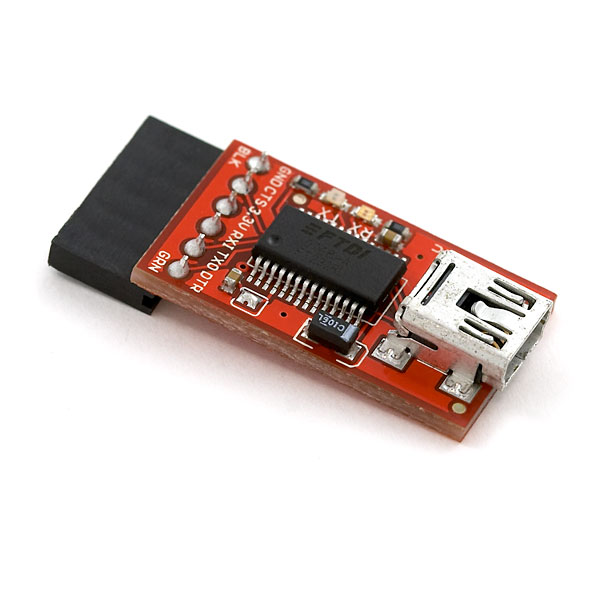
\includegraphics[scale=0.3]{pcb_ejemplo}
%\caption{PCB de ejemplo}\label{fig:pcb_ejemplo}
%\end{figure}

